\newpage

\section{Design}

\begin{comment}
 What is required for the Design Section:
 - Aesthetic Prototype ( CAD Images, photos of physical prototypes, drawings )
 - Design for Manufacture, Assembly, Maintenance
 - Block Diagrams
 - Wiring Diagrams
 - State Transition Diagrams
 - Technology ( languages, hardware, etc. )
 - Simulation
 - Modeling
\end{comment}

\subsection{Aesthetic Prototype}

Following extensive brainstorming and analysis, our team carefully evaluated a wide range of potential features and implementation strategies for our smart lock system. Ultimately, we selected the concept of using a solenoid-based locking mechanism controlled via a keypad and a smartphone app. This approach balanced feasibility, security, and user convenience. Our selection process included the use of the 6-3-5 method, which helped generate and refine a wide range of ideas across five categories: Hardware \& Mechanics, Smartphone Integration, Security Features, Software \& Control, and Advanced Features. We also brainstormed ideas of how the lock would potentially look like, for easy installation and fix up when an issue arises. All of our ideas were formed based on this appendix section: \ref{BrainstormingIdeas}.

\begin{figure}[!ht]
    \centering
    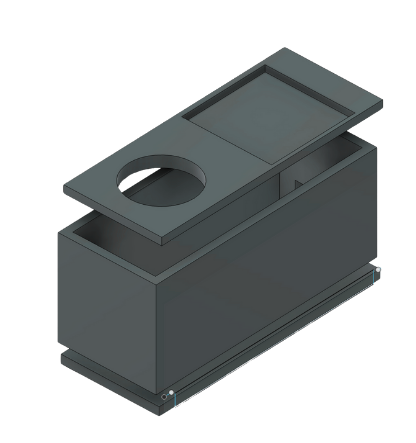
\includegraphics[width=0.80\textwidth]{img/AestheticPrototype.png}
    \caption{Aesthetic Prototype}
    \label{fig:aestheticPrototype}
\end{figure}

Figure \ref{fig:aestheticPrototype} illustrates our aesthetic prototype, which served as the foundation for the final functional prototype. The enclosure was designed to effectively house all internal components of the smart lock, including the circuit board and the ESP32-C3 module, while securely mounting the keypad on the exterior. Its design allowed for quick and simple assembly and provided clear visibility of the locking mechanism from the side, making it easy to identify whether the device was in the locked or unlocked state.

After 3D printing the casing and assembling the internal components, we arrived at the final prototype shown in Figure \ref{fig:testOutside}.

\begin{figure}[!ht]
\centering
\begin{subfigure}{.5\textwidth}
  \centering
  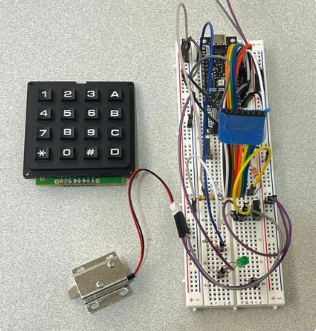
\includegraphics[width=.7\linewidth]{img/prototypeInside.png}
  \caption{Internal view of assembled prototype}
  \label{fig:pInside}
\end{subfigure}%
\begin{subfigure}{.5\textwidth}
  \centering
  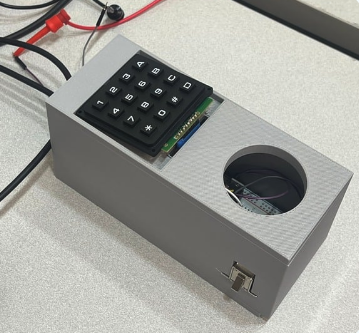
\includegraphics[width=.7\linewidth]{img/prototypeOutside.png}
  \caption{External view of assembled prototype}
  \label{fig:pOutside}
\end{subfigure}
\caption{Assembled functional prototype with 3D-printed casing}
\label{fig:testOutside}
\end{figure}

\subsection{Design for Manufacture, Assembly, Maintenance} % we need to add more detail from our previous work from 123A...read his comments from draft
\subsubsection*{Design For Manufacture}
Our Design for Manufacture (DFM) is illustrated in Figure~\ref{fig:DFM} below.

\begin{figure}[!ht]
    \centering
    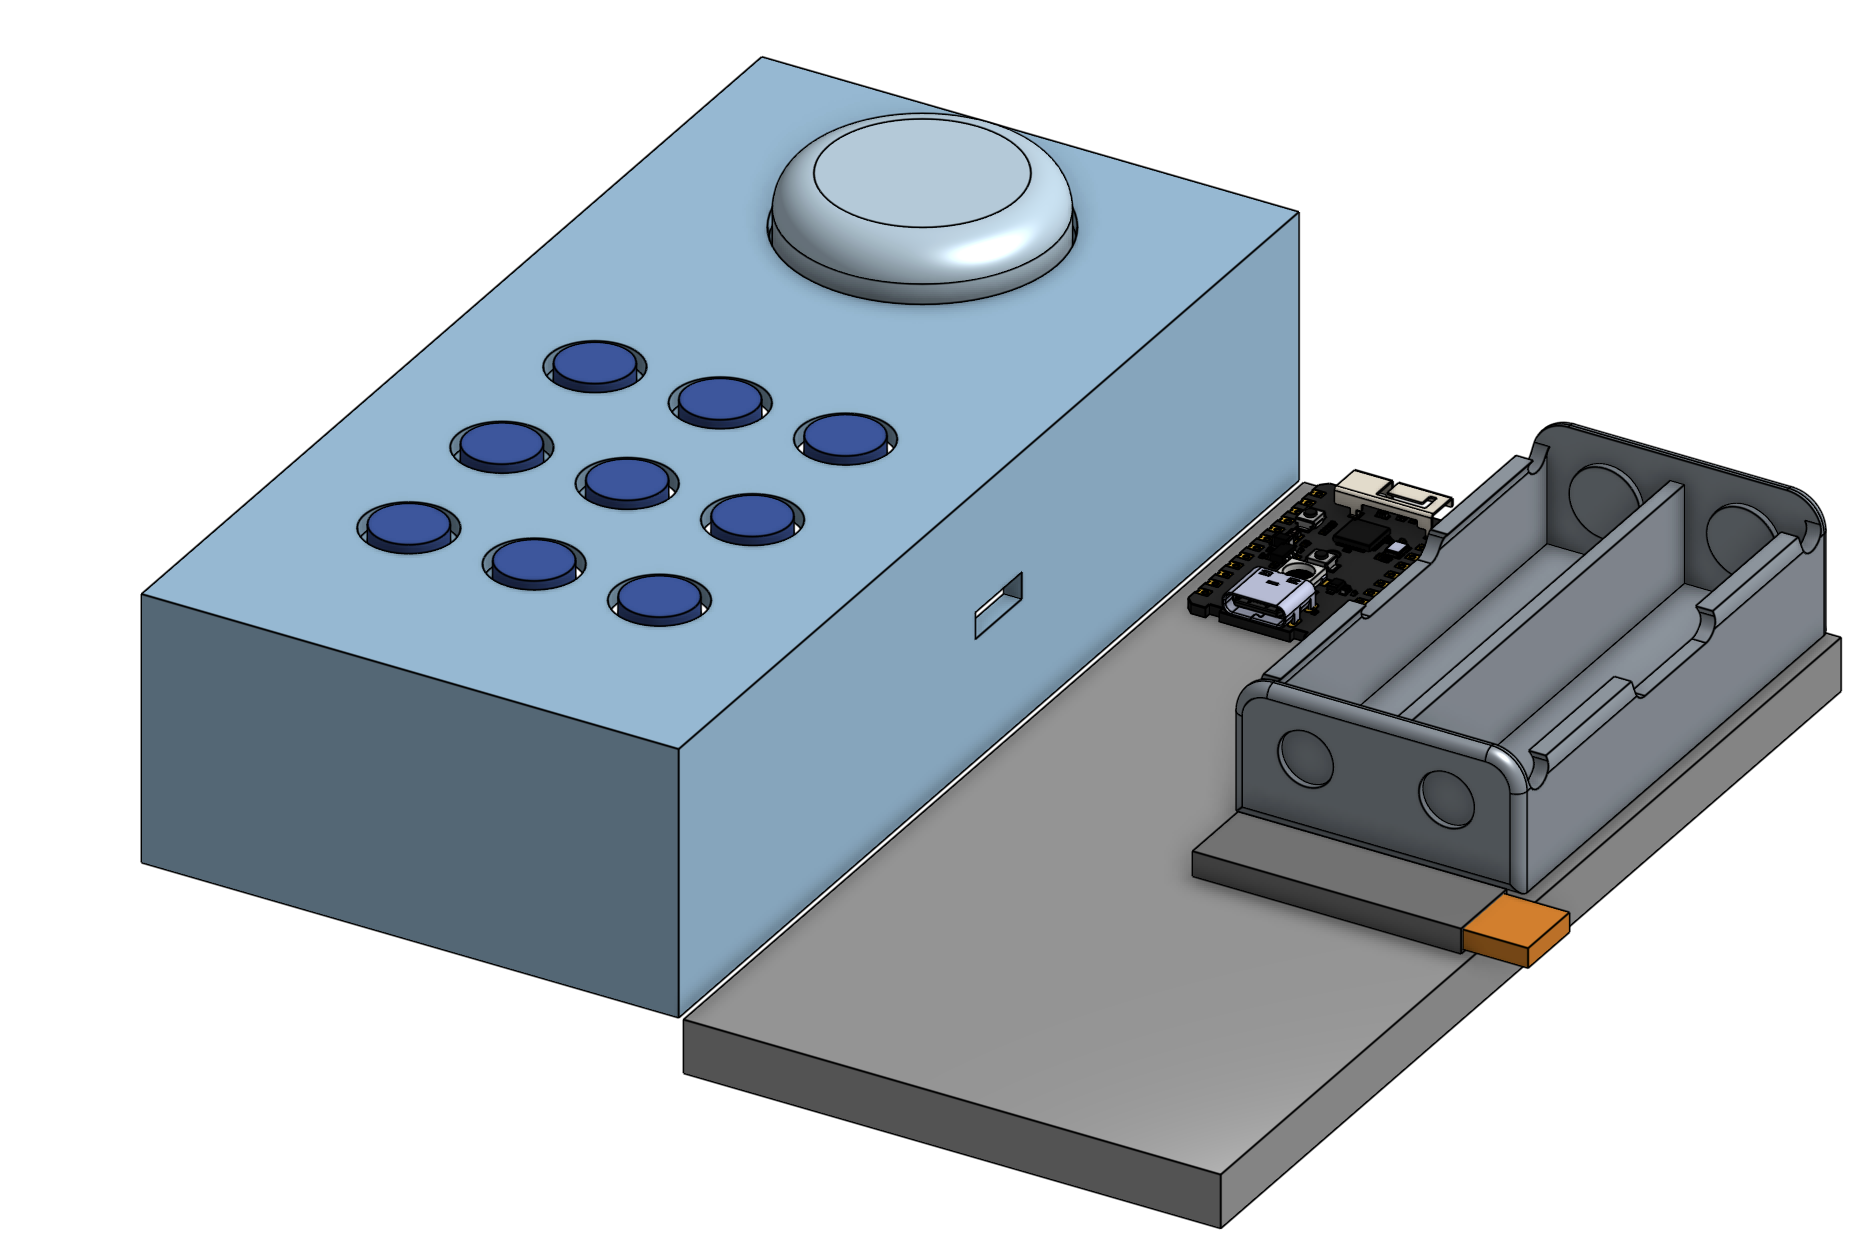
\includegraphics[width=0.80\textwidth]{img/DFM side view.png}
    \caption{DFM}
    \label{fig:DFM}
\end{figure}

As shown in the figure, the front of the device features an integrated keypad for primary user input, with space allocated for an additional module to support secondary authentication — enhancing security by verifying the identity of the user. Internally, the design houses the microcontroller, a rechargeable battery pack, and a solenoid lock mechanism.

The form factor has been developed with modern aesthetics and user-friendliness in mind, ensuring that the device is both visually appealing and intuitive for homeowners to operate. Component placement has also been optimized for efficient assembly, accessibility, and long-term maintainability.

\subsubsection*{Design For Assembly}
To ensure ease of assembly, our smart lock design emphasizes modular components, minimal fasteners, and intuitive alignment features. Figure~\ref{fig:DFA_Exploded} illustrates the exploded view of the product, showing the order and orientation of each major part during assembly.

\begin{figure}[!htbp]
    \centering
    \begin{subfigure}[b]{0.48\textwidth}
        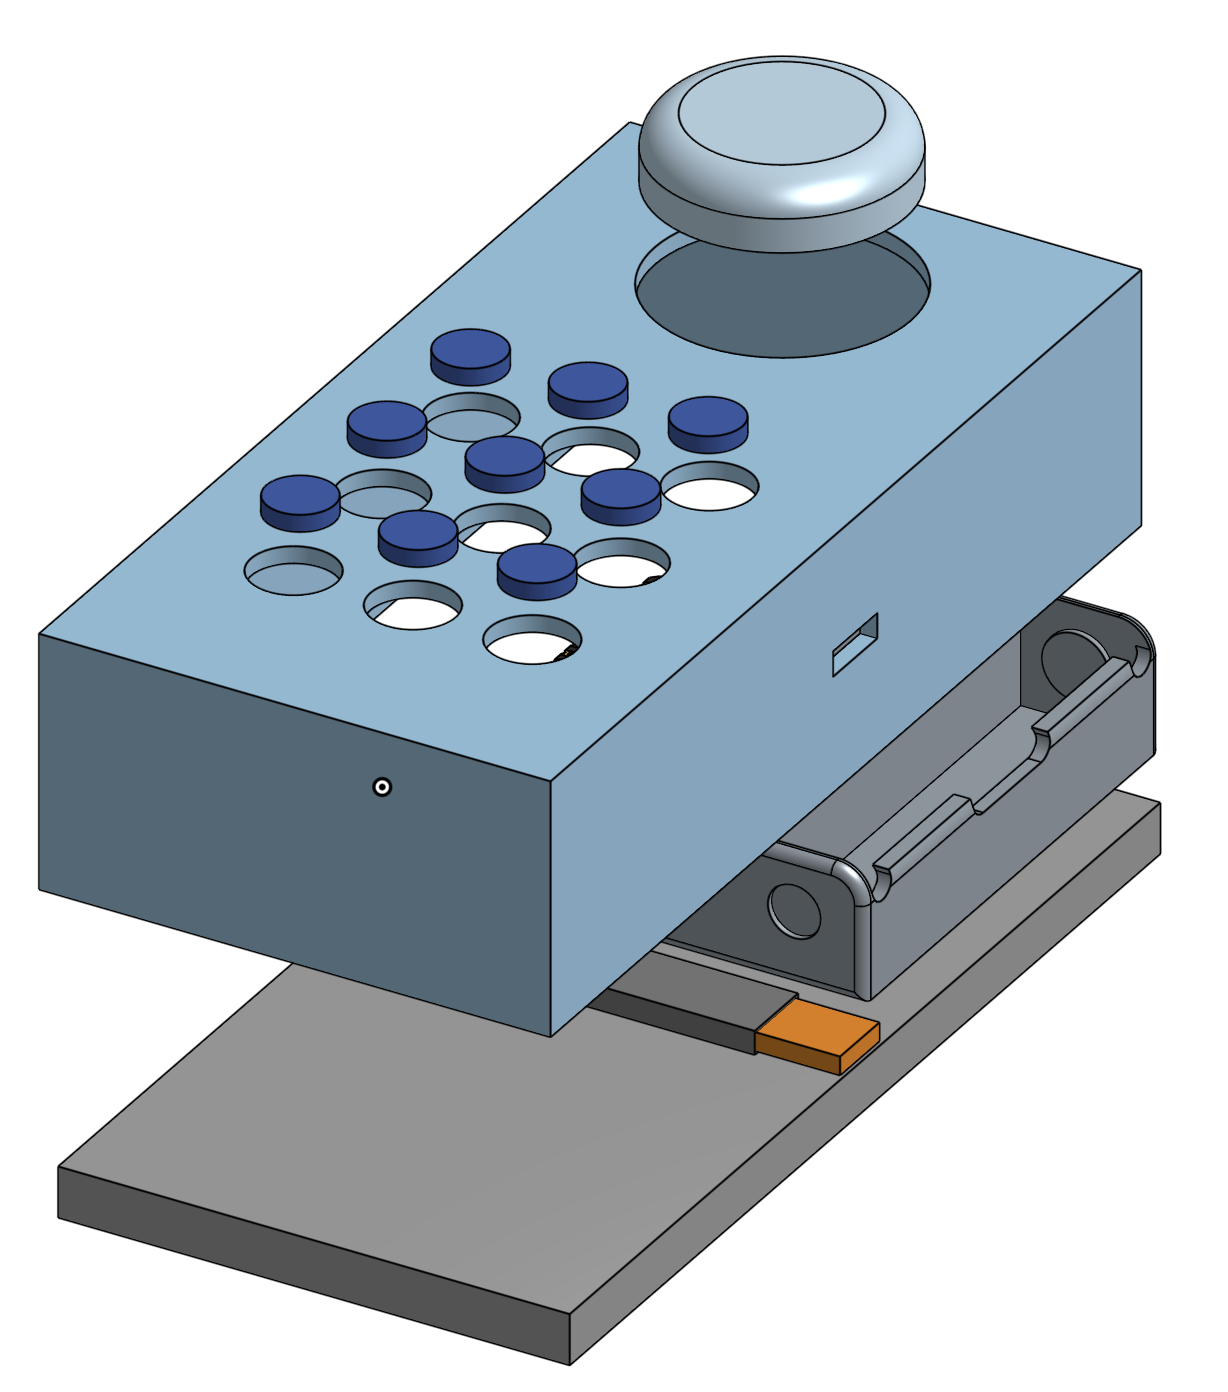
\includegraphics[width=\textwidth]{./img/DFA_Right.png}
        \caption{Exploded view right side}
        \label{fig:DFA_Right}
    \end{subfigure}
    \hfill
    \begin{subfigure}[b]{0.48\textwidth}
        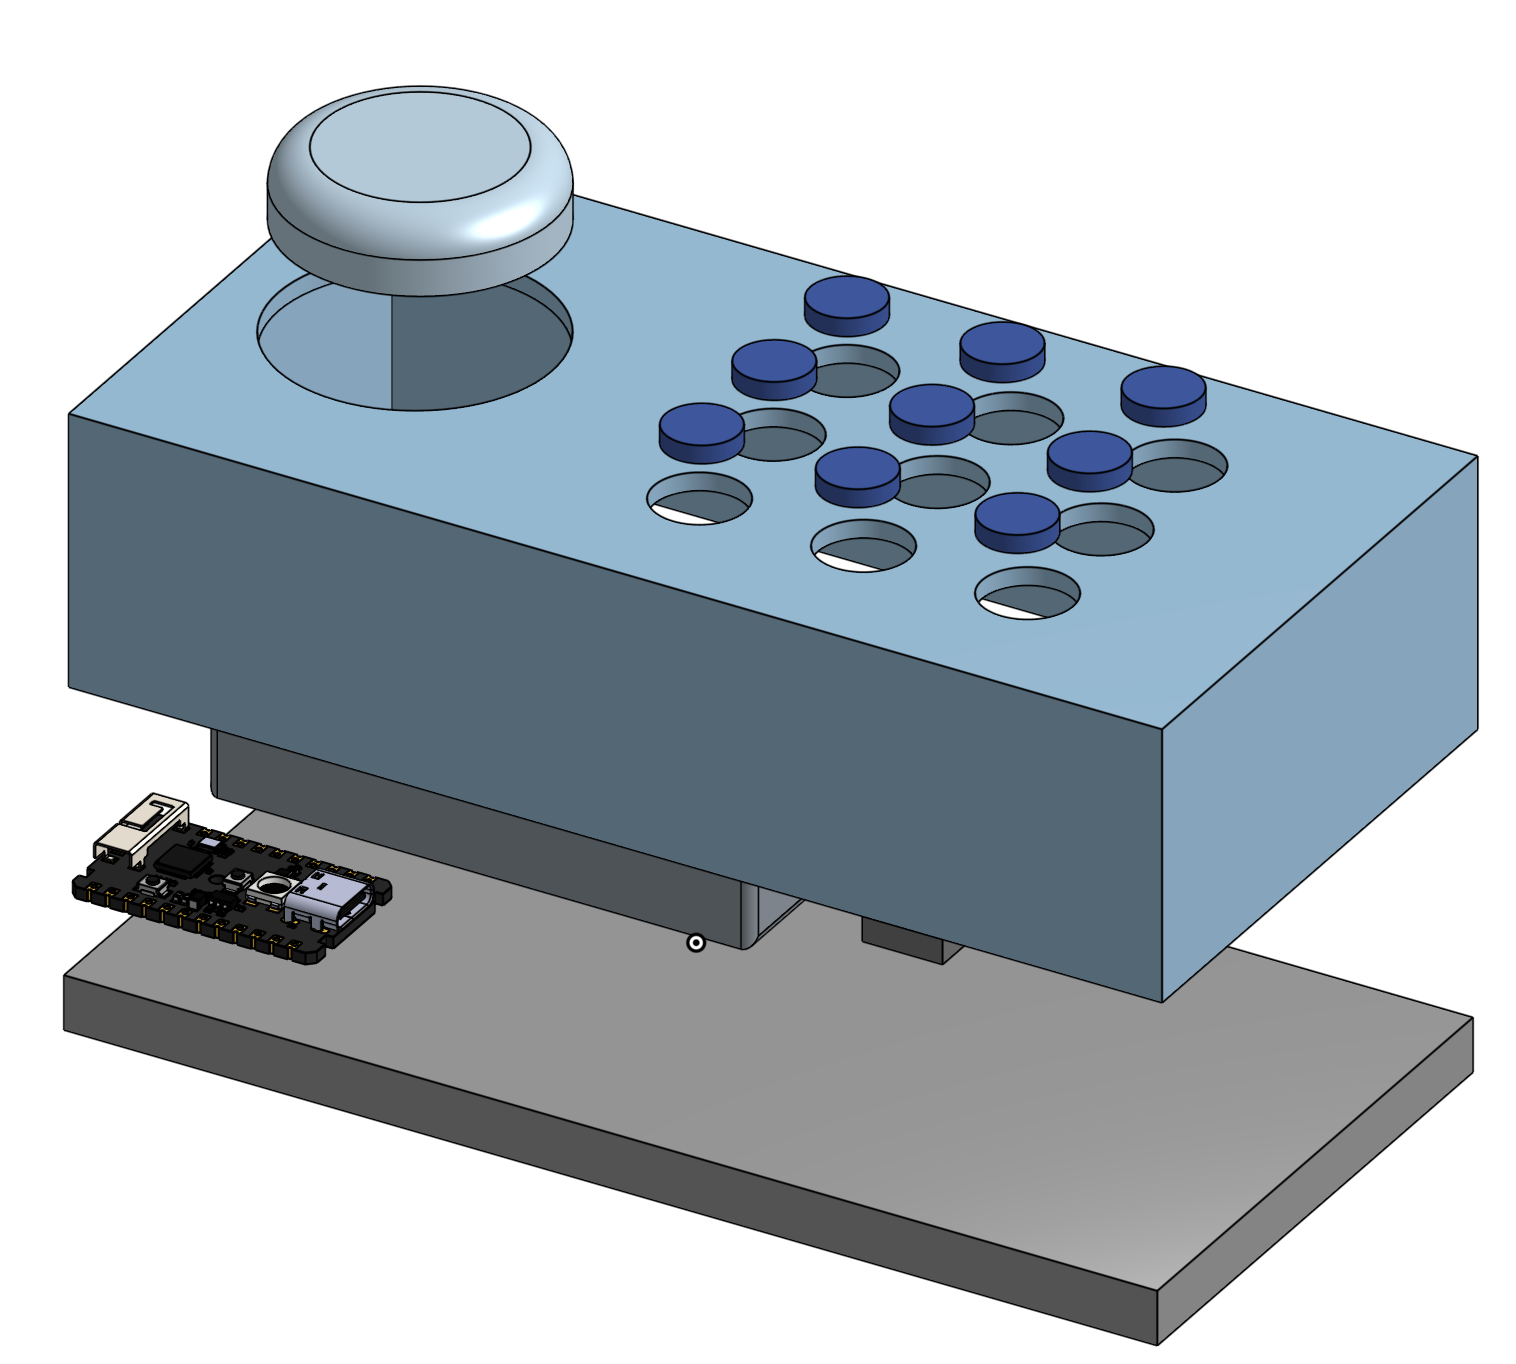
\includegraphics[width=\textwidth]{./img/DFA_Left.png}
        \caption{Exploded view left side}
        \label{fig:DFA_Left}
    \end{subfigure}
    \caption{First lock design}
    \label{fig:DFA_Exploded}
\end{figure}

The design separates the internal electronics (microcontroller, battery pack, and PCB) as a single sub-assembly that can be installed into the enclosure before final sealing. The keypad snaps into place on the front panel, and the housing is secured with four screws for quick final assembly. The overall approach minimizes assembly time and reduces the potential for user or manufacturing error.

\subsubsection*{Design for Maintenance}
The smart lock is engineered for long-term usability with minimal service requirements. A key feature of the design is the accessible battery compartment, which allows users to replace batteries without disassembling the entire unit. Standard Phillips screws secure the housing, avoiding the need for proprietary tools and simplifying field servicing.

Internally, components such as the microcontroller and solenoid lock are mounted modularly, allowing them to be replaced individually if a failure occurs. This modular approach extends the product's usable life and reduces electronic waste. Over-the-air (OTA) firmware updates are supported via the smartphone app, enabling remote bug fixes and feature updates without physical access.

Maintenance is further supported through built-in diagnostics: users receive alerts for low battery, Wi-Fi disconnection, or tampering, helping address issues before they escalate. The device is designed to operate reliably for several years with only basic battery replacement and no specialized maintenance.

\subsection{Block Diagrams}

For our block diagram, we will describe how we are going to connect our system together for our hardware, software, along with our server. The figure \ref{fig:blockDiagram} illustrates the entire system architecture. Starting from the left, we have the keypad that allows users to input access codes to control the locking mechanism. The keypad sends these inputs to the microcontroller, which acts as the central processing unit for the system.

\begin{figure}[ht]
    \centering
    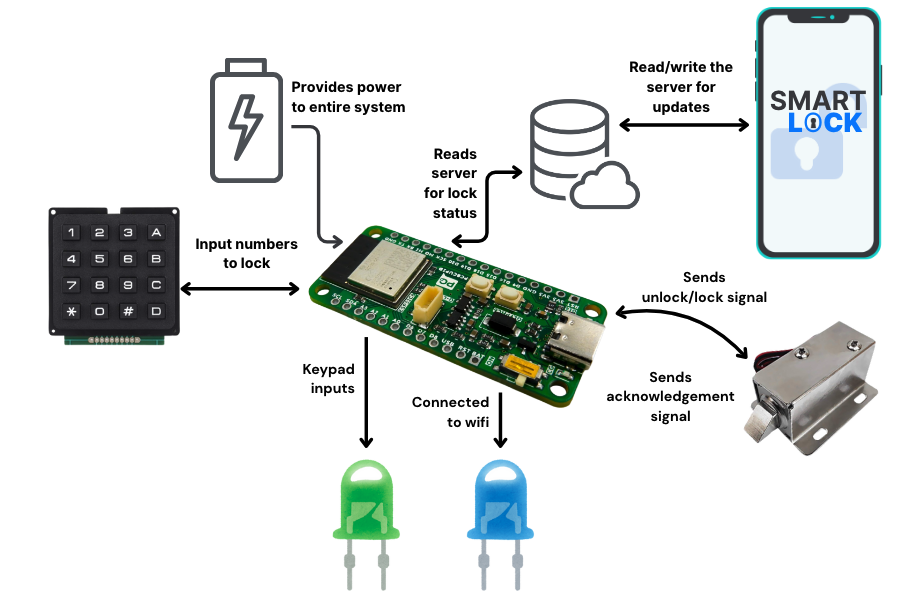
\includegraphics[width=0.80\textwidth]{img/blockDiagram.png}
    \caption{Block Diagram}
    \label{fig:blockDiagram}
\end{figure}

The microcontroller processes the user input and communicates with the solenoid lock to either engage or disengage the locking bolt based on the verification of the input code. Additionally, the microcontroller connects to the Wi-Fi module to enable remote communication with our server.

On the software side, the server hosts the backend services responsible for managing user authentication, storing access logs, and syncing lock states. It communicates with the microcontroller over the internet, allowing authorized users to control the lock remotely through a mobile application.

The mobile application serves as the user interface, enabling users to send lock or unlock commands, receive status updates, and manage access credentials. This client-server interaction ensures that users can securely control their smart lock from anywhere, while the system maintains real-time synchronization between hardware and software components.

Together, these interconnected blocks form a cohesive system that balances local authentication via the keypad with remote management through the server and mobile app, ensuring convenience and security.

\subsection{Wiring Diagrams}

In the wiring diagram shown in figure \ref{fig:wiringDiagram}, you can observe the specific pin connections between the ESP32-C3 microcontroller and the various hardware components in our system. These connections directly correspond to the GPIO (General Purpose Input/Output) pins configured in our firmware, ensuring that the software interfaces correctly with the physical devices.

\begin{figure}[ht]
    \centering
    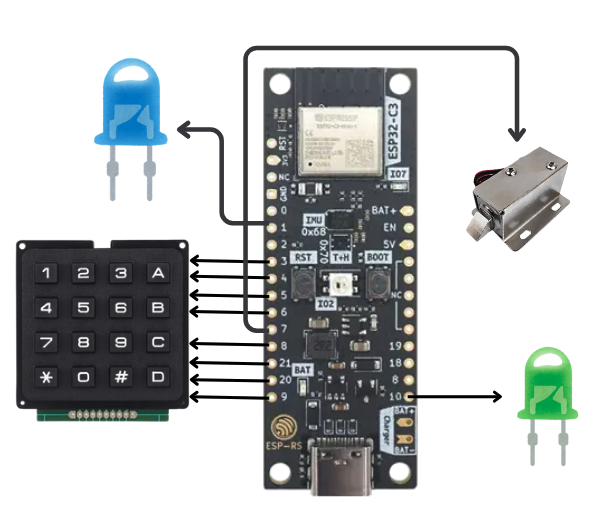
\includegraphics[width=0.80\textwidth]{img/wiringDiagram.png}
    \caption{Wiring Diagram}
    \label{fig:wiringDiagram}
\end{figure}

Starting with the keypad, each row and column line is connected to designated GPIO pins on the ESP32-C3, allowing the microcontroller to detect button presses through a matrix scanning method. This setup enables efficient reading of multiple keys with minimal pin usage. The solenoid lock control is wired to a digital output pin, which is driven high or low by the microcontroller to activate or deactivate the lock mechanism. A mosfet transistor is included in the circuit to handle the higher current required by the solenoid, protecting the ESP32-C3 from damage. Additionally, the ESP32-C3’s Wi-Fi antenna and power lines are properly connected to ensure stable wireless communication and device operation. Power supply lines are clearly marked, showing how the system components are powered, whether from an external source or regulated onboard power. The wiring diagram serves as a vital reference during assembly and troubleshooting, providing a clear mapping of all hardware interfaces. Correct adherence to this diagram ensures that the system components operate reliably and the software can control the hardware as intended.

\subsection{State Transition Diagrams}
Figure \ref{fig:stateTransitionDiagram} illustrates the state machine used in our smart lock system. This diagram outlines the various operational states of the system and the transitions between them, triggered by user inputs, system events, or remote commands.

\begin{figure}[ht]
    \centering
    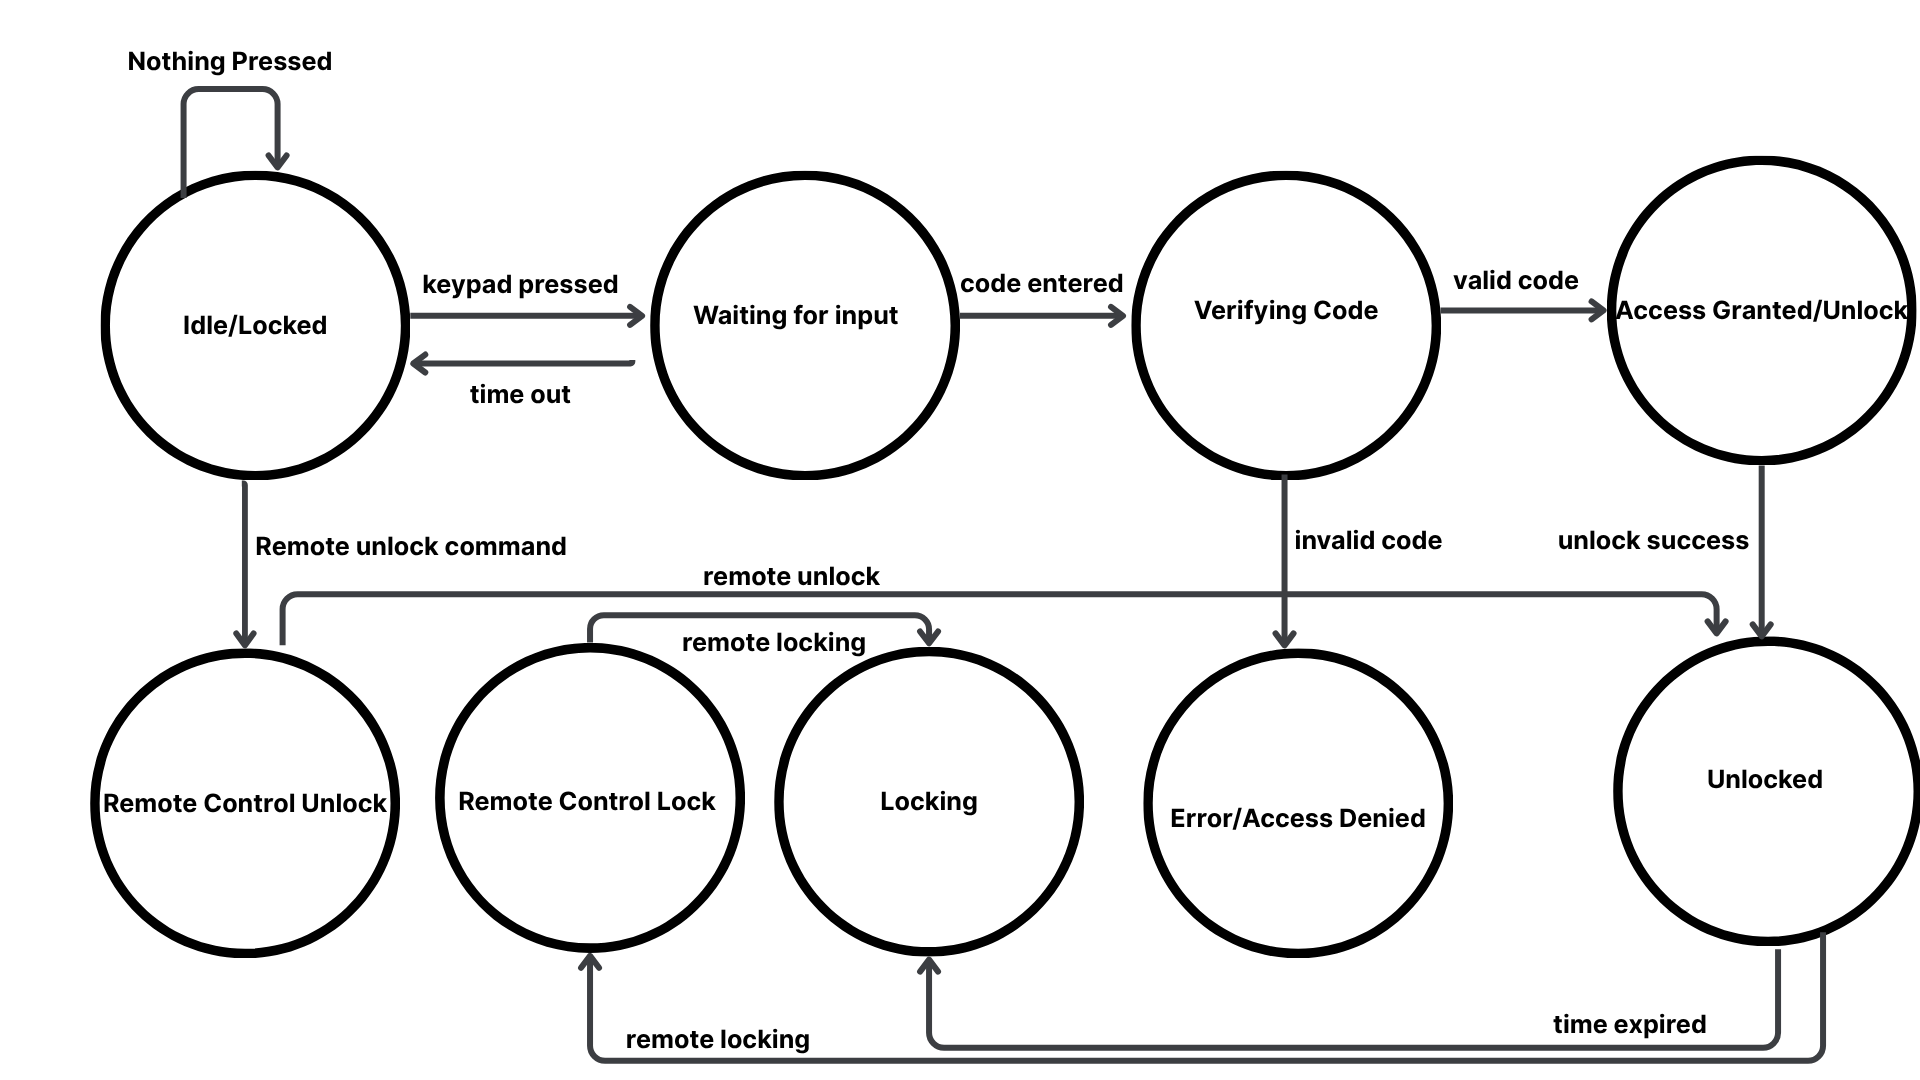
\includegraphics[width=0.80\textwidth]{img/stateTransitionDiagram.png}
    \caption{State Machine Diagram}
    \label{fig:stateTransitionDiagram}
\end{figure}

The system starts in the Idle/Locked state, where it remains until user interaction is detected. When a key is pressed on the keypad, the system transitions to the Waiting for Input state, where it captures the full access code. After the user submits a code, the system enters the Verifying Code state. At this point, the input is checked either locally or through server communication. If the code is valid, the system proceeds to the Access Granted / Unlocking state, where the solenoid is activated to unlock the door. Once unlocked, the system moves to the Unlocked state and remains there for a set duration to allow entry. After the timeout period, the system transitions to the Locking state, re-engaging the solenoid to secure the door, and finally returns to Idle/Locked. If the entered code is invalid, the system transitions to the Error / Access Denied state, providing feedback to the user (e.g., a buzzer or LED alert), before returning to Idle/Locked after a short delay. The system also supports remote interactions. A command from the mobile app can transition the system from Idle/Locked to Remote Control Unlocking, and from Unlocked to Remote Control Locking. These remote actions follow similar unlock and lock procedures as local interactions.

\subsection{Technology}
For our hardware components, we used the ESP32-C3 microcontroller, programmed in C++ using the Arduino IDE. To support our development, we integrated several key libraries: Firebase Client by Mobizt, ArduinoJson by Benoit Blanchon, WiFiManager by tzapu, and Keypad by Mark Stanley and Alexander Brevig. These libraries enabled reliable communication with our Firebase server, interfacing with the keypad for user input, and creating a Wi-Fi access point for initial smart lock configuration. 

As for the smartphone app, we used Swift with Xcode for development. This means that our application currently builds natively for iOS devices only, such as iPhones and iPads. The app allows users to unlock and lock the smart lock remotely, receive battery and connectivity status notifications, and manage temporary PIN codes.

While our current version supports iOS exclusively, we plan to explore cross-platform solutions such as Flutter or React Native in the future to make the app available on Android devices as well. This would broaden accessibility and improve compatibility for a wider range of users.

\subsection{Simulation}

To better understand the performance, reliability, and longevity of our smart lock system, we developed several system-level models: power consumption, timing responsiveness, and brute-force protection.

\textbf{Power Model:}  
We modeled the average power usage of the system based on both datasheet specifications and realistic use scenarios. In our optimized configuration, the ESP32-C3 remains in deep sleep mode (10~\textmu A) and only wakes on external interrupts (e.g., keypad input). During operation, the ESP32 briefly activates Wi-Fi and the solenoid for unlocking.

\begin{itemize}
    \item \textbf{Deep sleep:} 10~\textmu A for ~24 hours/day minus active time
    \item \textbf{Active mode:} 80~mA for 10 seconds per unlock (10 uses/day)
    \item \textbf{Solenoid:} 500~mA for 0.5 seconds per unlock
\end{itemize}

The total energy used per day is estimated as:
\[
\text{ESP32 (sleep)} \approx 0.0666~\text{mAh}, \quad
\text{ESP32 (active)} \approx 2.22~\text{mAh}, \quad
\text{Solenoid} \approx 0.694~\text{mAh}
\]
\[
P_{\text{daily}} \approx 2.98~\text{mAh/day}
\]

With a 3.7V 18650 Li-ion battery rated at 3,000~mAh, the expected runtime is:
\[
\text{Battery Life} = \frac{3,000~\text{mAh}}{2.98~\text{mAh/day}} \approx 1,007~\text{days} \approx \boxed{2.75~\text{years}}
\]

Factoring in losses due to regulators, temperature variation, and battery aging, a conservative real-world estimate is \textbf{1.5 to 2 years} of battery life per charge.

\textbf{Timing Model:}  
We modeled the response time from keypad input to unlocking to ensure a smooth user experience. Based on observed behavior and testing, the total average time is approximately 1.5 seconds:
\begin{itemize}
    \item Keypad entry: ~0.5 seconds
    \item Code verification (local/remote): ~0.3 seconds
    \item Solenoid activation and unlock: ~0.7 seconds
\end{itemize}

This timing model confirmed that our system remains responsive while conserving power.

\textbf{Security Model:}  
To mitigate brute-force attempts, we modeled the security of a 4-digit PIN system, which has 10,000 possible combinations. We implemented a lockout mechanism:
\begin{itemize}
    \item Maximum of 3 failed attempts before temporary lockout
    \item Lockout duration: 30 seconds
    \item Lockout resets after inactivity or power cycle
\end{itemize}

This simple model helps protect against unauthorized access while balancing usability.

These models helped guide hardware component choices (such as low-power microcontrollers and solenoid driver circuits), define software timing thresholds, and enforce robust security policies in our firmware design.

\subsection{Final Design}

\newpage
\subsection{Battery Power Management and Notification System}

While the prototype operates on a continuous power source, a commercial SmartLock will use a secure, long-lasting battery to ensure usability during power outages and in locations without fixed power. Proper battery management involves monitoring charge levels, notifying users, and providing a safe and secure method for recharging or replacing the battery.

\subsubsection{Battery Selection and Power Optimization}

Selecting the right battery type and minimizing power consumption are critical for long-term operation.

\begin{itemize}
  \item \textbf{Battery Type:} Use high-capacity rechargeable lithium-ion or lithium-polymer batteries capable of lasting several months on a single charge.
  \item \textbf{Low Power Modes:} Implement deep sleep and wake-on-interrupt features in the firmware to minimize power draw during idle periods.
\end{itemize}

\subsubsection{Battery Monitoring and User Notification}

Monitoring battery status and notifying users to ensure maintenance and avoid unexpected lockouts.

\begin{itemize}
  \item \textbf{Voltage Monitoring Circuit:} Integrate a voltage divider or dedicated battery management gauge to continuously monitor battery levels.
  \item \textbf{Battery State Logging:} Periodically upload battery status to the cloud alongside status logs.
  \item \textbf{User Notifications:} Send low battery alerts via push notifications, email, or in-app messages when battery drops below a critical threshold (e.g., 30\%).
\end{itemize}

\subsubsection{Safe and Secure Battery Replacement or Recharging}

Users must be able to service the battery safely without compromising lock security or usability.

\begin{itemize}
  \item \textbf{Secure Battery Access:} Design an internal battery compartment accessible only when the lock is in an unlocked state or with a secure override mechanism.
  \item \textbf{Rechargeable Design:} Provide a USB-C or magnetic charging port for easy recharging without disassembling the lock.
  \item \textbf{Tamper Detection:} Include log entries if the battery compartment is accessed, and notify the owner.
  \item \textbf{Backup Power Support:} Consider integrating a backup battery to retain state data during battery swap, or integrate a way to reset lock data upon battery replacement or recharge.
\end{itemize}


\subsection{Ownership and Access Control}

Managing ownership and granting user access are critical to ensuring that SmartLock devices remain secure while allowing for flexible sharing. This system must allow primary users to delegate lock access to other users, while ensuring that the delegated users have the appropriate permissions.

\subsubsection{Ownership Model}

Each SmartLock must have a primary owner who holds full control over the device and its permissions.

\begin{itemize}
  \item \textbf{Lock Registration:} When a new lock is initialized, the registering user becomes the owner.
  \item \textbf{Ownership Table:} Store ownership information in the database alongside lock records (e.g., \texttt{lock\_id}, \texttt{owner\_id}).
\end{itemize}

\subsubsection{Access Delegation and Permissions}

Primary owners can grant access to other users, allowing them to interact with specific locks under defined conditions.

\begin{itemize}
  \item \textbf{Access Table:} Maintain a table or collection with fields such as \texttt{lock\_id}, \texttt{user\_id}, \texttt{access\_level} (view, control), \texttt{granted\_by}, and \texttt{expiration} if necessary.
  \item \textbf{Access Rights Enforcement:} Backend logic and security rules should enforce permissions before allowing user actions.
  \item \textbf{Revocation and Expiration:} Include features for the owner to revoke access at any time or set expiration timers for temporary access.
\end{itemize}

\subsubsection{User Interface for Access Management}

The frontend application should allow users to manage and review access settings.

\begin{itemize}
  \item \textbf{Access Dashboard:} Display which users currently have access to a given lock and their permission levels.
  \item \textbf{Invite Flow:} Enable owners to invite users via email or user ID, specifying which lock(s) they can access.
\end{itemize}

%%%%%%%%%%%%%%%%%%%%%%%%%
%
%
% History and Logging
%
%
%%%%%%%%%%%%%%%%%%%%%%%%%

\newpage
\subsection{History and Status Logging}

 Logging improves security, aids in diagnostics, and enhances transparency for users. The SmartLock system should log both user actions and technical status changes.

\subsubsection{History Log of User Actions}

Tracking user interactions with locks helps in audits, diagnostics, and usage insights.

\begin{itemize}
  \item \textbf{Log Entry Fields:} Include \texttt{timestamp}, \texttt{user\_id}, \texttt{lock\_id}, and \texttt{action} (e.g., lock, unlock, access granted).
  \item \textbf{Database:} Automatically write to the history log whenever a user successfully executes an action.
  \item \textbf{User Access to Logs:} Allow users to view logs for locks they own or have access to.
\end{itemize}

\subsubsection{Status Log for Lock Health Monitoring}

Status logs are essential for monitoring device reliability and connectivity.

\begin{itemize}
  \item \textbf{Microcontroller Event Logging:} Program the microcontroller to push logs to Cloud structure or a backend data on significant events (e.g., Wi-Fi reconnect, battery low).
  \item \textbf{Technical Dashboard:} Visualize connection stability and firmware state for each lock.
\end{itemize}

\subsubsection{Action Confirmation and Notifications}

Users must be notified when actions are completed to reinforce trust and responsiveness.

\begin{itemize}
  \item \textbf{Action Acknowledgement:} ESP32 should confirm action execution back to Cloud database (e.g., “locked: true”).
  \item \textbf{Notification Service:} Use real-time updates to the mobile app or web interface.
  \item \textbf{Failure Alerts:} Alert users if an action fails, with details such as connectivity issues or mechanical faults.
\end{itemize}


%% Server Infrastructure %%

\subsubsection{Database and Server Infrastructure}

Figure \ref{fig:serverInfrasture} illustrates the many-to-many relationship within our server infrastructure design. In this architecture, a single user can be associated with multiple smart locks, and each lock can be controlled by multiple users. This flexible relationship model allows for shared access scenarios—such as families, property managers, or Airbnb hosts—where multiple authorized users may need to manage or access the same lock.

\begin{figure}[!ht]
    \centering
    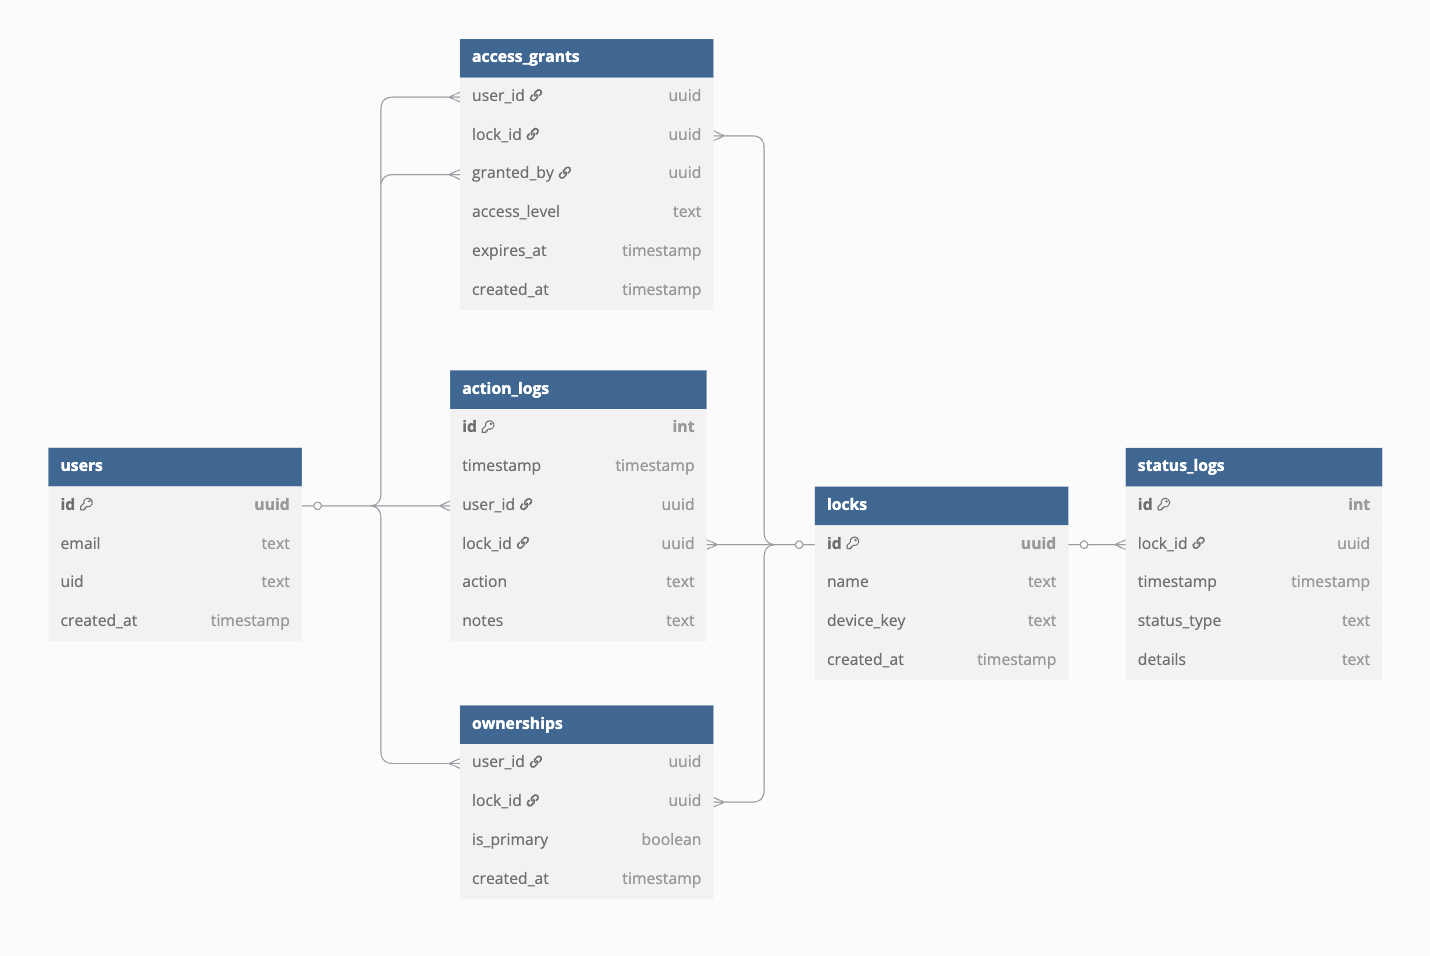
\includegraphics[width=0.65\textwidth]{img/serverInfrastructure.png}
    \caption{Server Infrastructure}
    \label{fig:serverInfrasture}
\end{figure}

The database schema is designed to support this many-to-many relationship efficiently through the use of a join table that links users and locks. This structure lays the foundation for scalable and secure access management in future implementations.

For our manufactured product, we plan to migrate from Firebase to a more robust backend using PostgreSQL for the database and Amazon Web Services (AWS) for cloud hosting and scalability. PostgreSQL is a powerful open-source relational database that offers strong support for complex queries, relationships, and data integrity—making it ideal for managing multiple users, locks, and their associations. Its flexibility and reliability are critical for handling real-world access control logic, audit logging, and time-based features such as PIN expiration.

AWS will provide the underlying infrastructure to host our backend services, offering high availability, global reach, and integration with other tools such as AWS Lambda, S3, and IAM for secure identity and access management. By leveraging AWS, we gain better control over security, performance, and scalability, all of which are essential for deploying a production-ready smart lock system that supports many users and devices.

This upgrade positions our system for commercial deployment while ensuring a secure, efficient, and maintainable server-side architecture.

%% Bluetooth sharing wifi %%

\subsubsection{Bluetooth Wi-Fi Provisioning}

In our current prototype, Wi-Fi provisioning is achieved by having the device temporarily act as a wireless access point. Users connect to this access point and enter their Wi-Fi credentials and API key through a web interface. While functional, this method introduces unnecessary complexity for end users and is not ideal for a consumer-ready product.

In the manufactured product, we plan to implement Bluetooth-based Wi-Fi provisioning using our custom microcontroller. During setup, users will connect to the device via Bluetooth through the mobile application. The app will then securely transmit the Wi-Fi credentials directly to the lock, allowing it to connect to the appropriate network without requiring the user to switch networks or open a separate interface.

This approach greatly simplifies the onboarding process and aligns with common smart home device setup standards. It enhances the user experience by making setup faster, more intuitive, and less prone to user error. Bluetooth provisioning also improves compatibility with a broader range of mobile devices and operating systems.

By transitioning to Bluetooth for initial network configuration, we aim to provide a seamless and user-friendly setup process that is better suited for deployment at scale.

%% Die Casting Case %%

\subsubsection{Die Casting Case}

As part of our manufactured product design, we plan to transition from 3D-printed enclosures to a die-cast metal casing. This upgrade is aimed at improving both the durability and aesthetic appeal of the smart lock.

Die casting allows us to produce a high-quality, uniform housing that can withstand daily use, environmental exposure, and tampering attempts more effectively than plastic prototypes. The use of metal, such as aluminum or zinc alloy, also adds a professional finish to the final product while enhancing the overall strength and lifespan of the device.

\begin{figure}[!ht]
\centering
\begin{subfigure}{.5\textwidth}
  \centering
  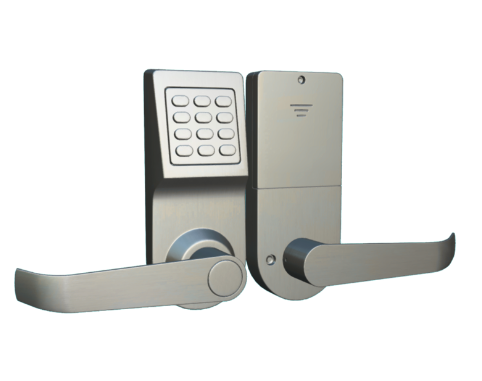
\includegraphics[width=.7\linewidth]{img/dieCast1.png}
  \caption{Die Cast Model}
  \label{fig:dieCast1}
\end{subfigure}%
\begin{subfigure}{.5\textwidth}
  \centering
  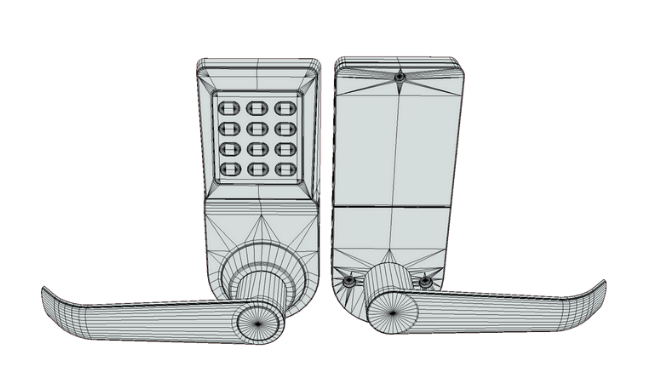
\includegraphics[width=.7\linewidth]{img/dieCast2.png}
  \caption{Sketch of Die Cast modell}
  \label{fig:dieCast2}
\end{subfigure}
\caption{Die Cast Casing}
\label{fig:dieCast}
\end{figure}

Figures \ref{fig:dieCast1} and \ref{fig:dieCast2} show our preliminary die-cast casing model and sketch. These designs reflect the key functional elements of the smart lock, including secure mounting points for the keypad, internal compartments for electronics, and a viewing area to indicate lock status. The internal layout was carefully designed to simplify assembly, minimize wiring complexity, and ensure heat dissipation where needed.

By adopting die casting for mass production, we ensure our product is manufacturable at scale while meeting real-world demands for security, reliability, and sleek appearance.